\section{Results}
\label{sec:results}

We report two pre-registered runs in increasing scope. Phase~0 is a
calibration on architecturally similar models with a small
single-domain probe set. Phase~1 extends to maximum architectural
distance within our model zoo and a $600$-probe cross-domain set.
Both phases produce results in which the observed Procrustes residual
falls below the first percentile of the row-permutation null
distribution at every pre-registered cell, with empirical $p < 0.001$
in each case.

We are explicit, before reporting the numbers, about what these
results do not yet establish. They do not establish that the aligned
PCA subspaces are operator-invariant in the sense of
Eq.~\eqref{eq:leakage}; they do not isolate compositional structure
from lexical or template structure (no lexical baseline was run); they
were obtained without train/test split (Procrustes was fit and
evaluated on the same probe set); the promised CKA cross-validation
\cite{kornblith2019similarity} was not computed in this paper despite
being committed in \S\ref{sec:methods}; and they do not control for
training-distribution overlap between the model pairs. Each gap is
catalogued in detail in \S\ref{sec:requiredwork}.

\subsection{Phase~0 Calibration}
\label{sec:results-phase0}

\paragraph{Models.} Phi-4-Reasoning-Plus (8-bit MLX, \texttt{phi3}
dispatch, $L_A = 40$, $d_A = 5120$) against Qwen3-4B (8-bit MLX,
\texttt{qwen3} dispatch, $L_B = 36$, $d_B = 2560$). Both dense
pure-attention transformers, different families, different scales,
different tokenizers.

\paragraph{Probe set.} $N = 96$ propositions drawn from the titles of
existing political-economy / categorial-architecture paper drafts in
the Sovereign research corpus, phrased as coherence-evaluation prompts
of the form ``Consider the following claim: \texttt{<title>}. Is this
a coherent proposition?'' Probes are short ($12$--$20$ tokens) and
topically narrow.

\paragraph{Result.} Table~\ref{tab:phase0} reports the Phase~0
result. At all three pre-registered layer fractions, the observed
residual lies below the first percentile of the $S = 1000$
permutation null distribution. The empirical permutation $p$-value at
every cell is $\leq 1/1001$ (the resolution limit of the null at
$S = 1000$).

\begin{figure}[h]
\centering
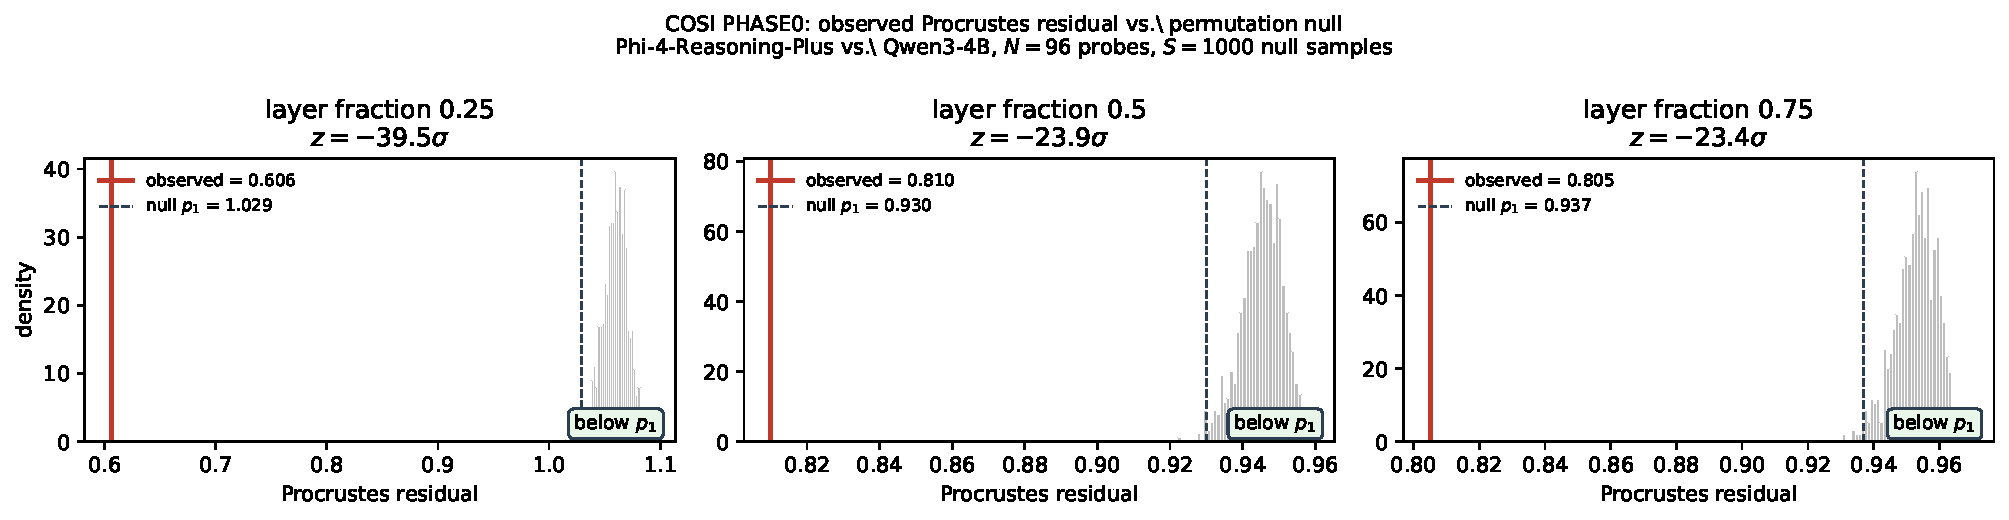
\includegraphics[width=\textwidth]{figures/phase0_residual_vs_null.pdf}
\caption{Phase~0 observed Procrustes residual (red vertical line)
against the permutation null distribution (gray histogram, $S = 1000$
samples) at three pre-registered layer fractions. The dashed black
line marks the first-percentile threshold of the null. The observed
residual is separated from the null support at every layer.}
\label{fig:phase0}
\end{figure}

\begin{table}[h]
\centering
\caption{Phase~0: Phi-4-Reasoning-Plus vs.\ Qwen3-4B,
$N = 96$ probes, $S = 1000$ permutation null samples per layer.
$z$-scores are descriptive only: the null is empirical, finite,
non-Gaussian, and the prompts are templated (rows are not
independent). Empirical permutation $p \leq 0.001$ at every cell.}
\label{tab:phase0}
\begin{tabular}{l c c c c r}
\toprule
Layer & $k$ & Residual & Perm.\ null mean ($\pm$ std) & Perm.\ null $p_1$ & Descriptive $z$ \\
\midrule
$0.25$ & $33$ & $0.6064$ & $1.0594$ ($\pm 0.011$) & $1.0292$ & $-39.54$ \\
$0.50$ & $27$ & $0.8100$ & $0.9453$ ($\pm 0.006$) & $0.9301$ & $-23.93$ \\
$0.75$ & $25$ & $0.8050$ & $0.9531$ ($\pm 0.006$) & $0.9369$ & $-23.42$ \\
\bottomrule
\end{tabular}
\end{table}

\paragraph{On the $z$-score language.} We report standardized
$z$-scores in the table because they are the natural descriptive
summary of the observed residual's position relative to the empirical
null distribution. We do \emph{not} interpret these as Gaussian
significance levels. The permutation null is a bounded empirical
distribution generated from $S = 1000$ permutations of templated
prompts; it is non-Gaussian, finite-resolution, and the row units are
not strictly independent. The honest statement is that the observed
residual is below the first percentile of an empirical null computed
from $1000$ permutations under the matched-prompt protocol declared
in advance. Whether the magnitude of the gap is scientifically
meaningful is a question the lexical baseline (Study B,
\S\ref{sec:requiredwork}) is required to answer.

\paragraph{Phase~0 pre-registration compliance.} The result satisfies
the pre-registered protocol declared in the companion design note
(\texttt{2026-05-06\_cosi\_design.md}, \S8) before observing data:
chance baselines computed on randomized inputs, layer fractions
$\{0.25, 0.5, 0.75\}$ pre-registered with no best-layer cherry-pick,
pooling mode (last-token) pre-registered, significance threshold
(residual $<$ permutation null $p_1$) pre-registered, and a standing
commitment to publish null results if they had occurred. We note that
the pre-registration document is committed to a private working
repository and is not externally timestamped; this is a known gap
addressed in Study G (\S\ref{sec:requiredwork}).

\subsection{Phase~1: Architectural Distance and Cross-Domain Probe Set}
\label{sec:results-phase1}

\paragraph{Models.} Phi-4-Reasoning-Plus (as Phase~0) against
Qwen3-Next-80B-A3B-Thinking (5-bit MLX, \texttt{qwen3\_next} dispatch,
$L_B = 48$, $d_B = 2048$, hybrid attention/state-space-model
architecture). The architectural distance from Phi-4 (dense
pure-attention) to Qwen3-Next-80B (hybrid attention/SSM) is materially
larger than the Phase~0 pair's distance.

\paragraph{Probe set.} $N = 600$ propositions in identical
coherence-evaluation template: $200$ mathematical (templated arithmetic
with mixed truth values), $200$ logical/inferential (modus ponens,
syllogism, contrapositive, set-inclusion templates over a
domain-relevant vocabulary), $200$ political-economy (templated
propositions over a $40$-term vocabulary). Generated with seed
$20260506$. Probes remain short ($12$--$30$ tokens).

\paragraph{Full-set result.} Table~\ref{tab:phase1-full} reports the
full-set alignment. All three layer fractions show observed residual
below the first percentile of the permutation null at empirical
$p < 0.001$.

\begin{table}[h]
\centering
\caption{Phase~1 full-set: Phi-4-Reasoning-Plus vs.\
Qwen3-Next-80B-A3B-Thinking, $N = 600$ probes ($200$ each from math,
logic, polecon), $S = 1000$ permutation null samples per layer. Same
caveats on $z$-score interpretation as Table~\ref{tab:phase0}.}
\label{tab:phase1-full}
\begin{tabular}{l c c c c r}
\toprule
Layer & $k$ & Residual & Perm.\ null mean ($\pm$ std) & Perm.\ null $p_1$ & Descriptive $z$ \\
\midrule
$0.25$ & $21$ & $0.7668$ & $1.0076$ ($\pm 0.011$) & $1.0004$ & $-101.00$ \\
$0.50$ & $25$ & $0.9056$ & $0.9943$ ($\pm 0.006$) & $0.9917$ & $-94.09$ \\
$0.75$ & $21$ & $0.9555$ & $0.9959$ ($\pm 0.005$) & $0.9947$ & $-88.55$ \\
\bottomrule
\end{tabular}
\end{table}

\begin{figure}[h]
\centering
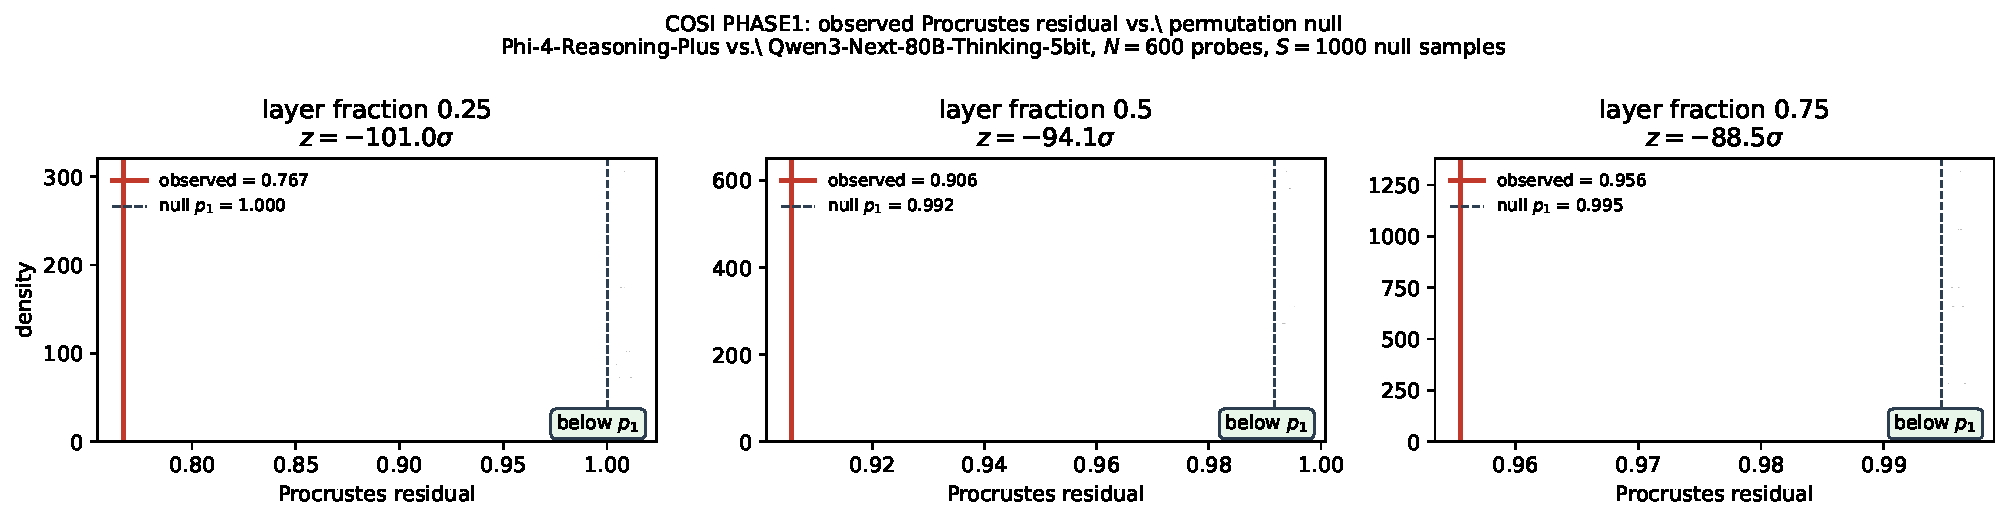
\includegraphics[width=\textwidth]{figures/phase1_residual_vs_null.pdf}
\caption{Phase~1 observed Procrustes residual (red vertical line)
against the permutation null distribution (gray histogram; $200$
samples shown for visualization, with summary statistics from the full
$S = 1000$ run). Same caveats as Phase~0.}
\label{fig:phase1-full}
\end{figure}

\paragraph{Per-domain stratification.} Table~\ref{tab:phase1-domain}
reports the alignment within each individual domain ($n = 200$ each,
$500$ permutation null samples per cell). All nine cells satisfy the
pre-registered significance criterion.

\begin{table}[h]
\centering
\caption{Phase~1 per-domain stratification ($n = 200$ each, $S = 500$
permutation null samples). Same caveats on $z$-score interpretation.}
\label{tab:phase1-domain}
\begin{tabular}{l l c c c r c}
\toprule
Domain & Layer & $k$ & Residual & Perm.\ null mean & Descriptive $z$ & Verdict \\
\midrule
math & $0.25$ & $8$ & $0.7473$ & $0.9962$ & $-56.40$ & below $p_1$ \\
math & $0.50$ & $10$ & $0.9010$ & $0.9886$ & $-49.57$ & below $p_1$ \\
math & $0.75$ & $8$ & $0.9535$ & $0.9933$ & $-38.76$ & below $p_1$ \\
logic & $0.25$ & $34$ & $0.8049$ & $0.9657$ & $-66.97$ & below $p_1$ \\
logic & $0.50$ & $45$ & $0.9158$ & $0.9755$ & $-60.58$ & below $p_1$ \\
logic & $0.75$ & $31$ & $0.9613$ & $0.9890$ & $-45.42$ & below $p_1$ \\
polecon & $0.25$ & $27$ & $0.8007$ & $0.9691$ & $-72.46$ & below $p_1$ \\
polecon & $0.50$ & $21$ & $0.9430$ & $0.9876$ & $-49.64$ & below $p_1$ \\
polecon & $0.75$ & $19$ & $0.9730$ & $0.9938$ & $-40.42$ & below $p_1$ \\
\bottomrule
\end{tabular}
\end{table}

\begin{figure}[h]
\centering
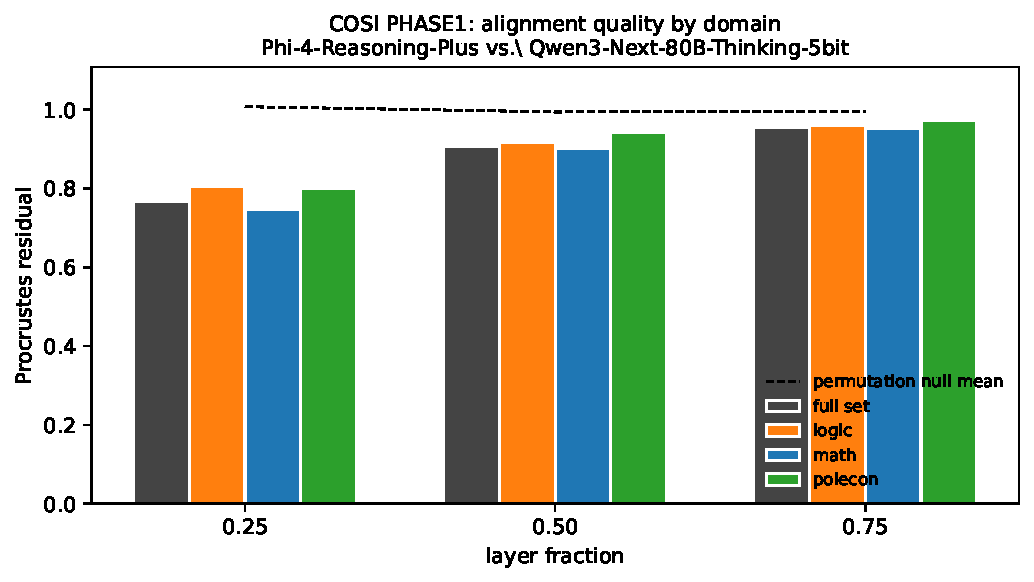
\includegraphics[width=0.85\textwidth]{figures/phase1_residual_by_domain.pdf}
\caption{Phase~1 alignment by domain at each layer fraction. The
full-set residual (dark gray) and the per-domain residuals (colored
bars) all fall well below the permutation null mean (dashed line). The
math-domain subspace dimension ($k = 8$--$10$) is substantially
smaller than the logic ($k = 31$--$45$) or polecon ($k = 19$--$27$)
subspaces. The dimensional difference is itself a substantive
empirical observation, but its operator-theoretic significance depends
on the invariance-leakage measurement (Study A,
\S\ref{sec:requiredwork}) which the present paper does not provide.}
\label{fig:phase1-domain}
\end{figure}

\subsection{Three Observations, Stated Carefully}

\paragraph{Observation 1: monotonic depth dependence.} The pattern of
residual increasing with layer depth (residual at $0.25 < 0.5 < 0.75$)
holds at the full-set level and within every domain. This is the most
robust pattern in the data. Three readings are consistent with it:
(\emph{i}) the operator-theoretic reading (early layers contain more
of the substrate-shared invariant subspace); (\emph{ii}) a
lexical-syntactic reading (early layers preserve token-level lexical
structure across vocabularies more than late layers preserve
task-specific computation); (\emph{iii}) a pooling-artifact reading
(last-token pooling at short prompt length is biased toward the
late-prompt syntactic state, which may be more architecture-shared
early in the network and more architecture-specific late). The pilot
does not discriminate among these. The pooling sweep (Study F) is
required to discriminate (\emph{iii}); the lexical baselines (Study B)
are required to discriminate (\emph{ii}).

\paragraph{Observation 2: domain-dependent subspace dimensionality.}
The PCA-derived $k$ at the $0.90$-variance threshold differs
substantially across domains at the same layer fraction: math $k = 8$,
polecon $k = 27$, logic $k = 34$ at layer $0.25$. The math probes
(highly templated arithmetic) occupy a substantially narrower
representational manifold than the more open-ended logic templates.
This is a substantive empirical observation that is consistent with
the variational/information-bottleneck framing
\cite{tishby2015deep, friston2010free, achille2018emergence}, but the
inference from ``low-dimensional PCA subspace'' to ``compositional
complexity is low'' requires whitening and fixed-$k$ controls (Study
F) and direct measurement of which subspace dimensions are
operator-invariant (Study A). Stated minimally: the PCA dimensionality
that captures $0.90$ of variance varies with domain in the predicted
direction.

\paragraph{Observation 3: relationship between Phase~0 and Phase~1.}
Phase~1's observed residuals are absolutely larger than Phase~0's
($0.77$ vs.\ $0.61$ at layer $0.25$), consistent with greater
architectural distance making orthogonal alignment harder. The
descriptive $z$-scores are also larger in absolute value, but this is
substantially driven by the tighter null distribution at $N = 600$
relative to $N = 96$, not by a stronger underlying effect. The
permutation null mean shifts from $1.06$ at $N = 96$ to $1.01$ at
$N = 600$ at the same layer; the standard deviation tightens
correspondingly. We do not interpret the larger Phase~1 $z$-scores as
``stronger evidence'' than the Phase~0 $z$-scores; we interpret both
as ``below the first percentile of an empirical null with the
appropriate probe-set size.''

\paragraph{Phase~1 pre-registration compliance.} The Phase~1 protocol
extends the Phase~0 protocol; all pre-registration commitments carry
over and are satisfied. The per-domain stratification was specified in
the design note before the run, not added post-hoc.
